
\section{Discussion and Conclusions}

The main research goal of the proposed activities is to evaluate and compare the different available versions for CVM-S4 velocity models. In order to do that, series of simuations are done for the under study velocity models and 30 moderate magnitude events located in the simulation domain. The GOF scores are calculated for them and the validation results condensed here statistically to facilitate their analysis. Fig.~\ref{fig:gof.avg.all} shows the average GOF scores for all the events, for each velocity model. Here, the average scores are obtained as the simple arithmetic mean of the GOF scores (FS values) from all the stations for each event. CVM-S4.26.223 is the most consistent model to yield the highest scores, between all four models. Also in this figure, we include a table on the margin with single-value scores for the velocity models. These are obtained by averaging the mean scores of all events for each model. Although once averaged, the differences between the values become marginal, they are consistent with the individual and overall mean values of each event. That is, the top score (4.87)corresponds to CVM-S4.26.223, followed by CVM-S4.26.222, CVM-S4.26.221, and CVM-S4.00. These observations are also consistent with the equivalent analysis when done based on the GOF scores obtained for broadband and the different frequency bands analysis. Our results for the goodness-of fit measure of the synthetics indicate that, CVMS4.26.223 shows an overall improvement for all the events.   


\begin{figure*}
    \centering
    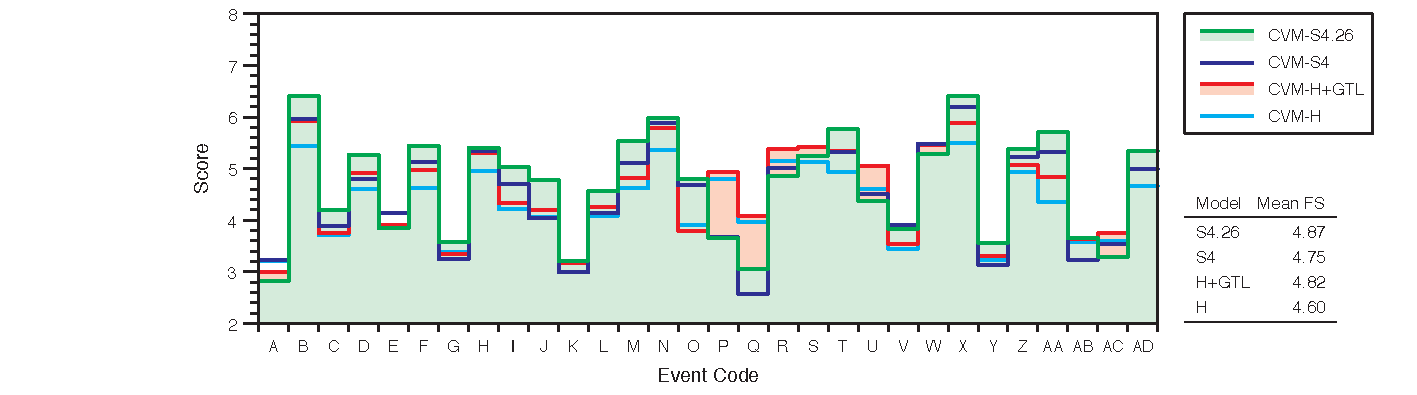
\includegraphics
        [width=\textwidth]
        {figures/pdf/figure-06}
    \caption{Summary of GOF results for all events. Values correspond to the average FS scores of all stations, in all components and frequency bands, discretized by velocity models. The values in the table to the right correspond to the mean value of the score for each velocity model considering all events. The areas under the lines for the values obtained with simulations using the velocity models CVM-S4.26.223, CVM-S4.26.222, CVM-S4.26.221 and CVM-4 are filled to highlight that CVM-S4.26.223 yields the largest number of events with the top value.}
    \label{fig:gof.avg.all}
\end{figure*}